\documentclass[conference]{IEEEtran}
\usepackage{times}
\usepackage{algorithm}
\usepackage{algpseudocode}
\usepackage{subfigure}
\usepackage{graphicx}
\usepackage{subfloat}
\usepackage{amsmath,empheq}
\usepackage{amssymb}
\usepackage{latexsym}

% numbers option provides compact numerical references in the text. 
\usepackage[numbers]{natbib}
\usepackage{multicol}
\usepackage[bookmarks=true]{hyperref}
\usepackage[usenames,dvipsnames]{color}
\newcommand{\stnote}[1]{\textcolor{Blue}{\textbf{ST: #1}}}
\newcommand{\dnote}[1]{\textcolor{Green}{\textbf{D: #1}}}
\newcommand{\gnote}[1]{\textcolor{Purple}{\textbf{G: #1}}}

\pdfinfo{
   /Author (David Abel  & Gabriel Barth-Maron, James MacGlashan, Stefanie Tellex)
   /Title  (Affordace-Aware Planning)
   /CreationDate (D:20101201120000)
   /Subject (Planning, Affordances, Sequential Decision Making)
   /Keywords (Planning, Affordance, MDP, Learning)
}

\begin{document}

% paper title
\title{Affordance-Aware Planning}

% You will get a Paper-ID when submitting a pdf file to the conference system
\author{Paper-ID [add your ID here]}

%\author{\authorblockN{Michael Shell}
%\authorblockA{School of Electrical and\\Computer Engineering\\
%Georgia Institute of Technology\\
%Atlanta, Georgia 30332--0250\\
%Email: mshell@ece.gatech.edu}
%\and
%\authorblockN{Homer Simpson}
%\authorblockA{Twentieth Century Fox\\
%Springfield, USA\\
%Email: homer@thesimpsons.com}
%\and
%\authorblockN{James Kirk\\ and Montgomery Scott}
%\authorblockA{Starfleet Academy\\
%San Francisco, California 96678-2391\\
%Telephone: (800) 555--1212\\
%Fax: (888) 555--1212}}


% avoiding spaces at the end of the author lines is not a problem with
% conference papers because we don't use \thanks or \IEEEmembership


% for over three affiliations, or if they all won't fit within the width
% of the page, use this alternative format:
% 
%\author{\authorblockN{Michael Shell\authorrefmark{1},
%Homer Simpson\authorrefmark{2},
%James Kirk\authorrefmark{3}, 
%Montgomery Scott\authorrefmark{3} and
%Eldon Tyrell\authorrefmark{4}}
%\authorblockA{\authorrefmark{1}School of Electrical and Computer Engineering\\
%Georgia Institute of Technology,
%Atlanta, Georgia 30332--0250\\ Email: mshell@ece.gatech.edu}
%\authorblockA{\authorrefmark{2}Twentieth Century Fox, Springfield, USA\\
%Email: homer@thesimpsons.com}
%\authorblockA{\authorrefmark{3}Starfleet Academy, San Francisco, California 96678-2391\\
%Telephone: (800) 555--1212, Fax: (888) 555--1212}
%\authorblockA{\authorrefmark{4}Tyrell Inc., 123 Replicant Street, Los Angeles, California 90210--4321}}


\maketitle

\begin{abstract}
Planning algorithms for non-deterministic domains are often
intractable in large state spaces due to the well-known ``curse of
dimensionality.'' Existing approaches to address this problem fail to
prevent the planner from considering many actions which would be
obviously irrelevant to a human solving the same problem.  We
formalize the notion of affordances~\citep{gibson77} as knowledge
added to an MDP that prunes actions in a state- and reward- general
way. This pruning significantly reduces the number of state-action
pairs the agent needs to evaluate in order to act optimally. We
demonstrate our approach in the Minecraft domain, showing significant
increase in speed and reduction in state-space exploration compared to
the standard versions of these algorithms. Further, we provide a
learning framework that enables an agent to learn affordances through
experience, removing the agent's dependence on the expert. We provide
preliminary results indicating that the learning process effectively
produces affordances that help solve an MDP faster.
\end{abstract}

\IEEEpeerreviewmaketitle

% ====== Section: Introduction ======
\section{Introduction}
\label{sec:introduction}
As robots move out of the lab and into the real world, planning
algorithms need to scale to domains of increased noise, size, and
complexity.  A classic formalization of this problem is a stochastic
sequential decision making problem in which the agent must find a
policy (a mapping from states to actions) for some subset of the state
space that enables the agent to achieve a goal from some initial
state, while minimizing any costs along the way.
Increases in planning problem size and complexity directly correspond
to an explosion in the state-action space. Current approaches to solving 
sequential decision making problems in the face of uncertainty cannot tackle these problems 
as the state-action space becomes too large~\citep{grounds05}.

To address this state-space explosion, prior work has explored adding
knowledge to the planner to solve problems in these
massive domains, such as options~\citep{sutton99} and
macroactions~\citep{Botea:2005kx,Newton:2005vn}. However, these
approaches add knowledge in the form of additional high-level actions
to the agent, which {\em increases} the size of the state-action space
(while also allowing the agent to search more deeply within the
space).  The resulting augmented space is even larger, which can have
the paradoxical effect of increasing the search time for a good
policy. Further, other approaches fall short of learning useful, transferable knowledge,
either due to complexity or lack of generalizability.

Instead, we propose a formalization of {\em affordances} \citep{gibson77} that enables an agent to focus on
aspects of the environment that are most relevant toward solving its current goal. Our approach avoids exploration of irrelevant parts of the 
state-action space, which leads to dramatic speedups in planning.

We formalize the notion of an affordance as a piece of planning
knowledge provided to an agent operating in a Markov Decision
Process (MDP). Further, we propose a learning process that
enables agents to autonomously learn affordances through experience, lessening
the agent's dependence on expert knowledge. Affordances are not specific to a particular reward 
function or state space, and thus, provide the agent with transferable 
knowledge that is effective in a wide variety of problems. 

Because affordances
define the {\em kind} of goals for which actions are useful,
affordances also enable high-level reasoning that can
be combined with approaches like high-level subgoal planning for even
greater performance gains. For now, we have chosen to ignore the direct 
perception of affordances in the environment, and have instead opted to emphasize an
affordance's ability to direct a planning agent through large stochastic state spaces. We foresee
future methods that incorporate vision and perception solutions with affordance-aware planners
to create robust, near-autonomous robotic agents.

% ====== Section: Background ======
\section{Background}
\label{sec:background}
We use Minecraft as our planning and evaluation domain. Minecraft is a
3-D blocks world game in which the user can place and destroy blocks
of different types.  Minecraft's physics and action space is expressive
enough to allow very complex worlds to be created by users, such as a
functional scientific graphing calculator\footnote{https://www.youtube.com/watch?v=wgJfVRhotlQ};
simple scenes from a Minecraft world appear in Figure~\ref{fig:epicworld} - a video demonstration of our system may be seen online\footnote{Watch at: https://vimeo.com/88689171}. Minecraft serves as a model for robotic tasks such as cooking assistance, assembling items in a factory, and object retrieval.  As in these tasks,  the agent operates in a very large state-action space in an uncertain environment.


\begin{figure*}
\centering
\subfigure[Start]{
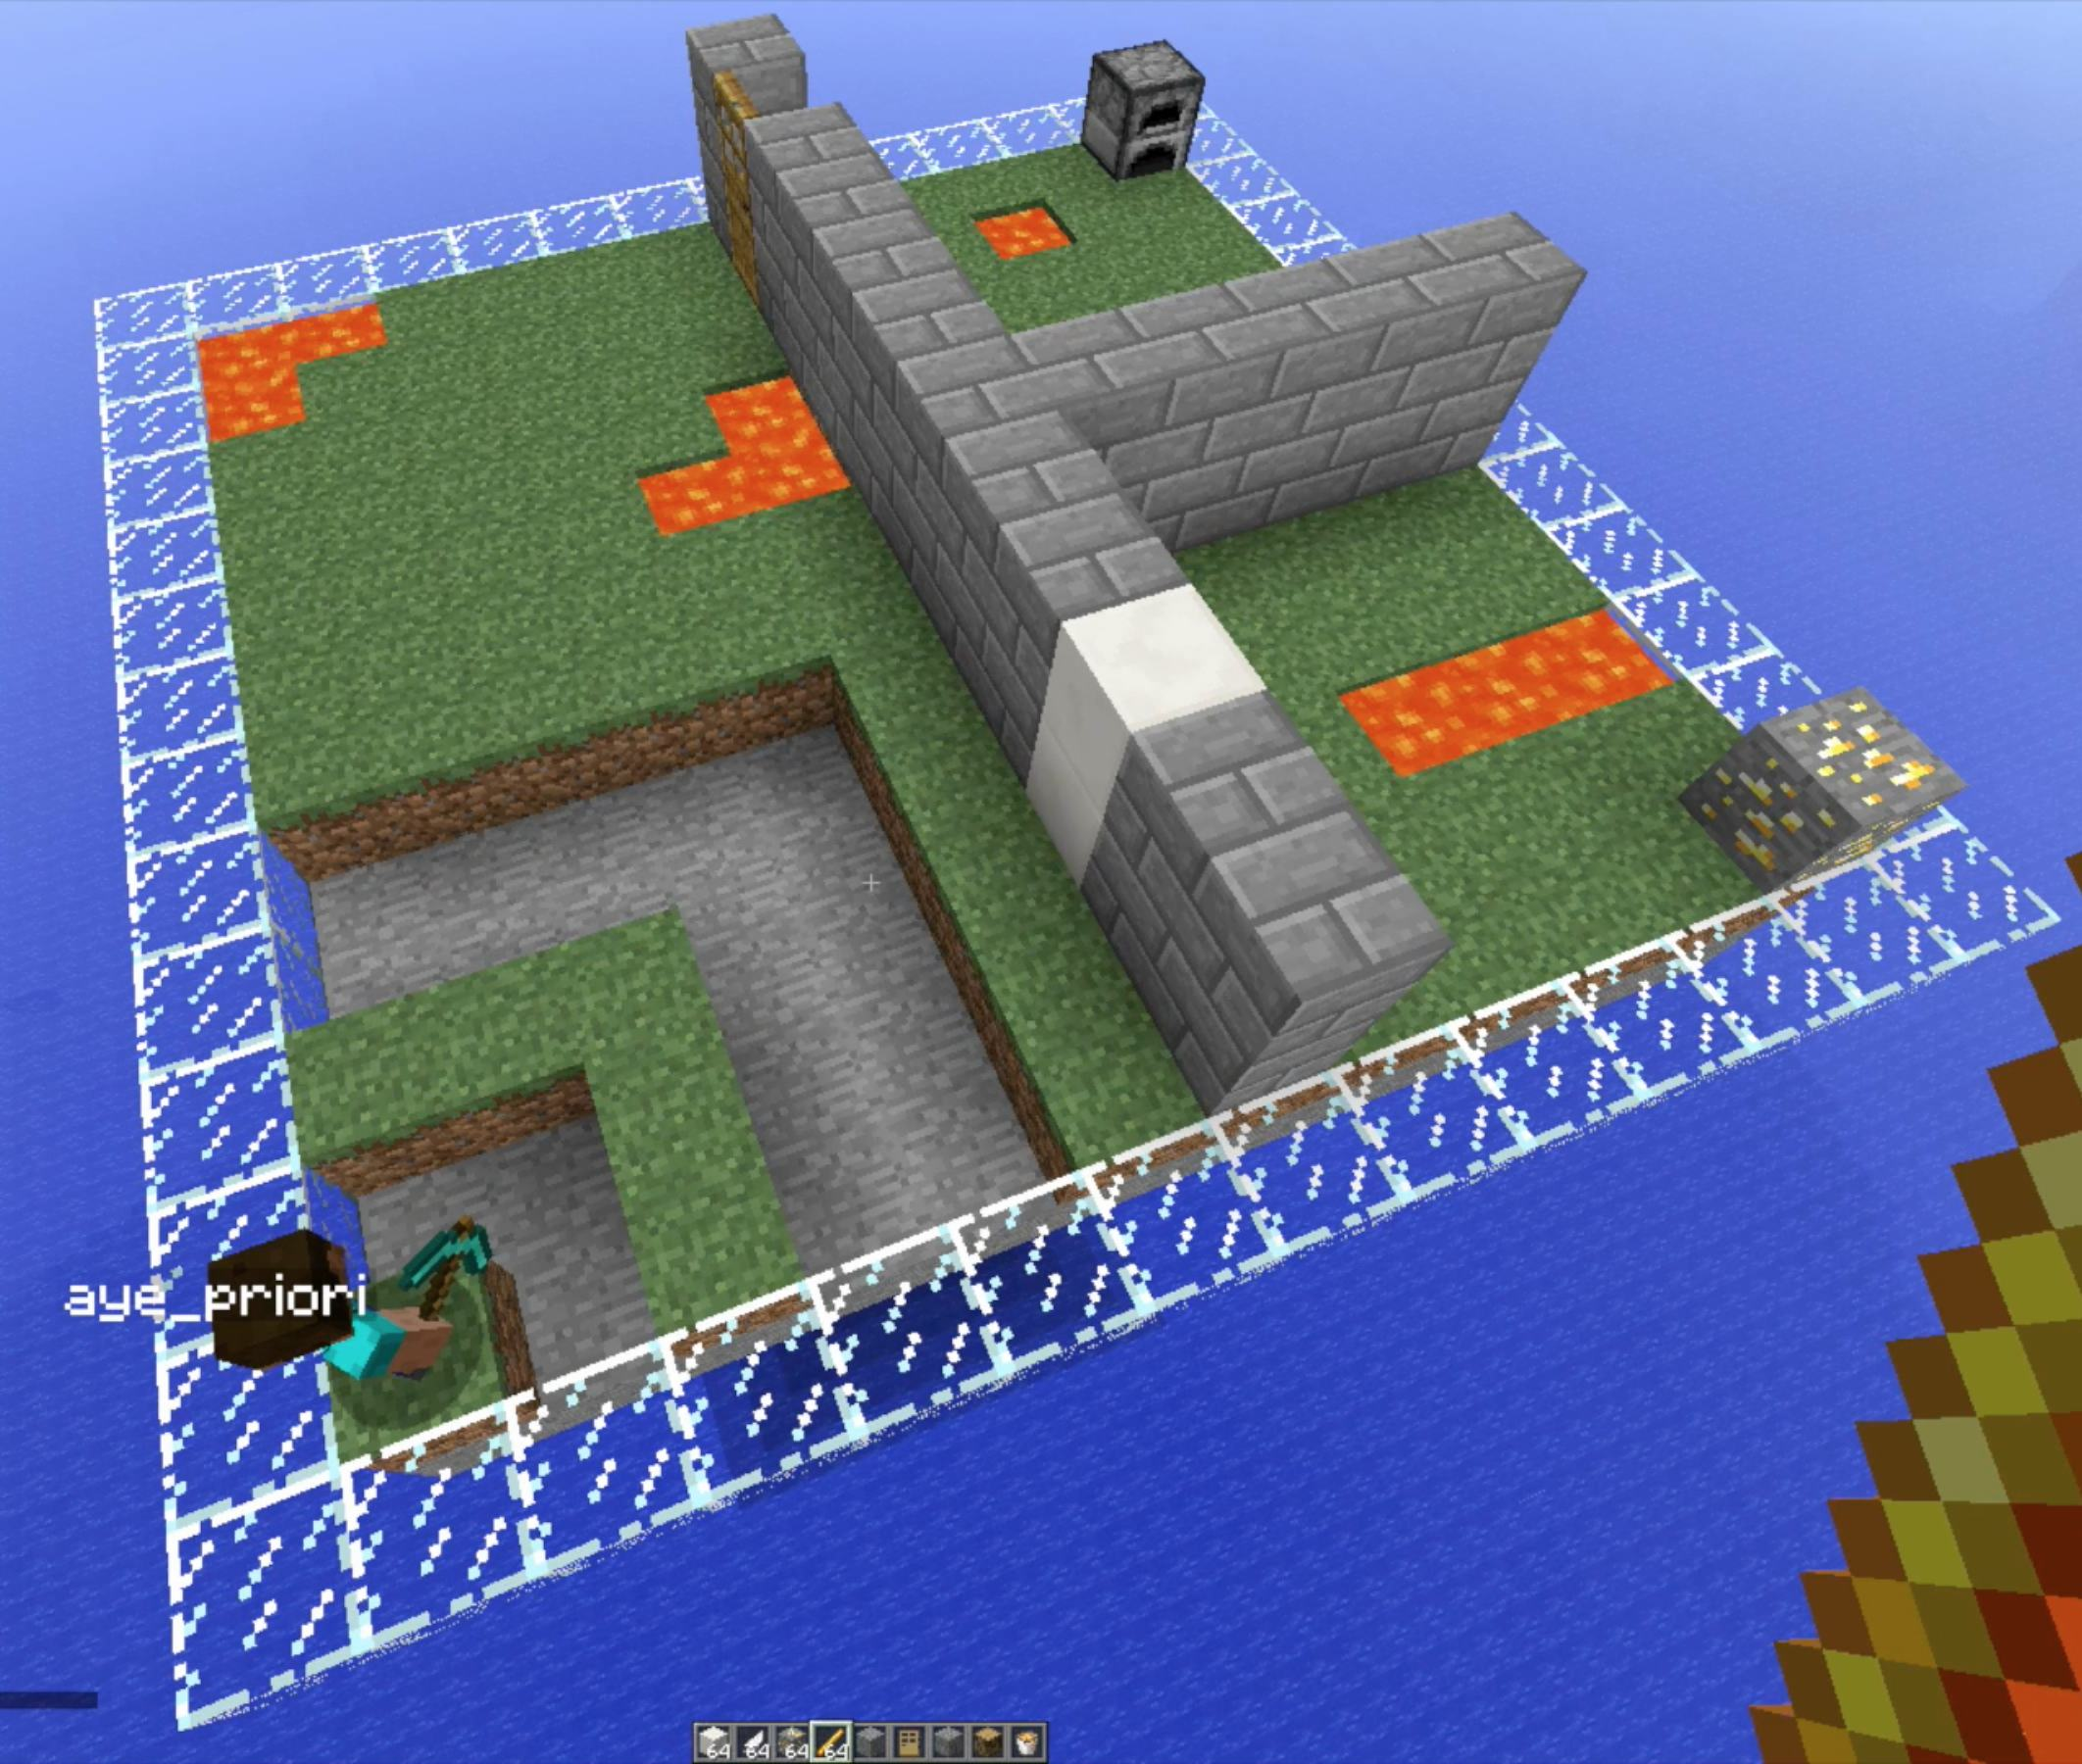
\includegraphics[width=0.24\linewidth]{figures/epicworld_1.jpg}}%
\subfigure[Destroy Wall]{
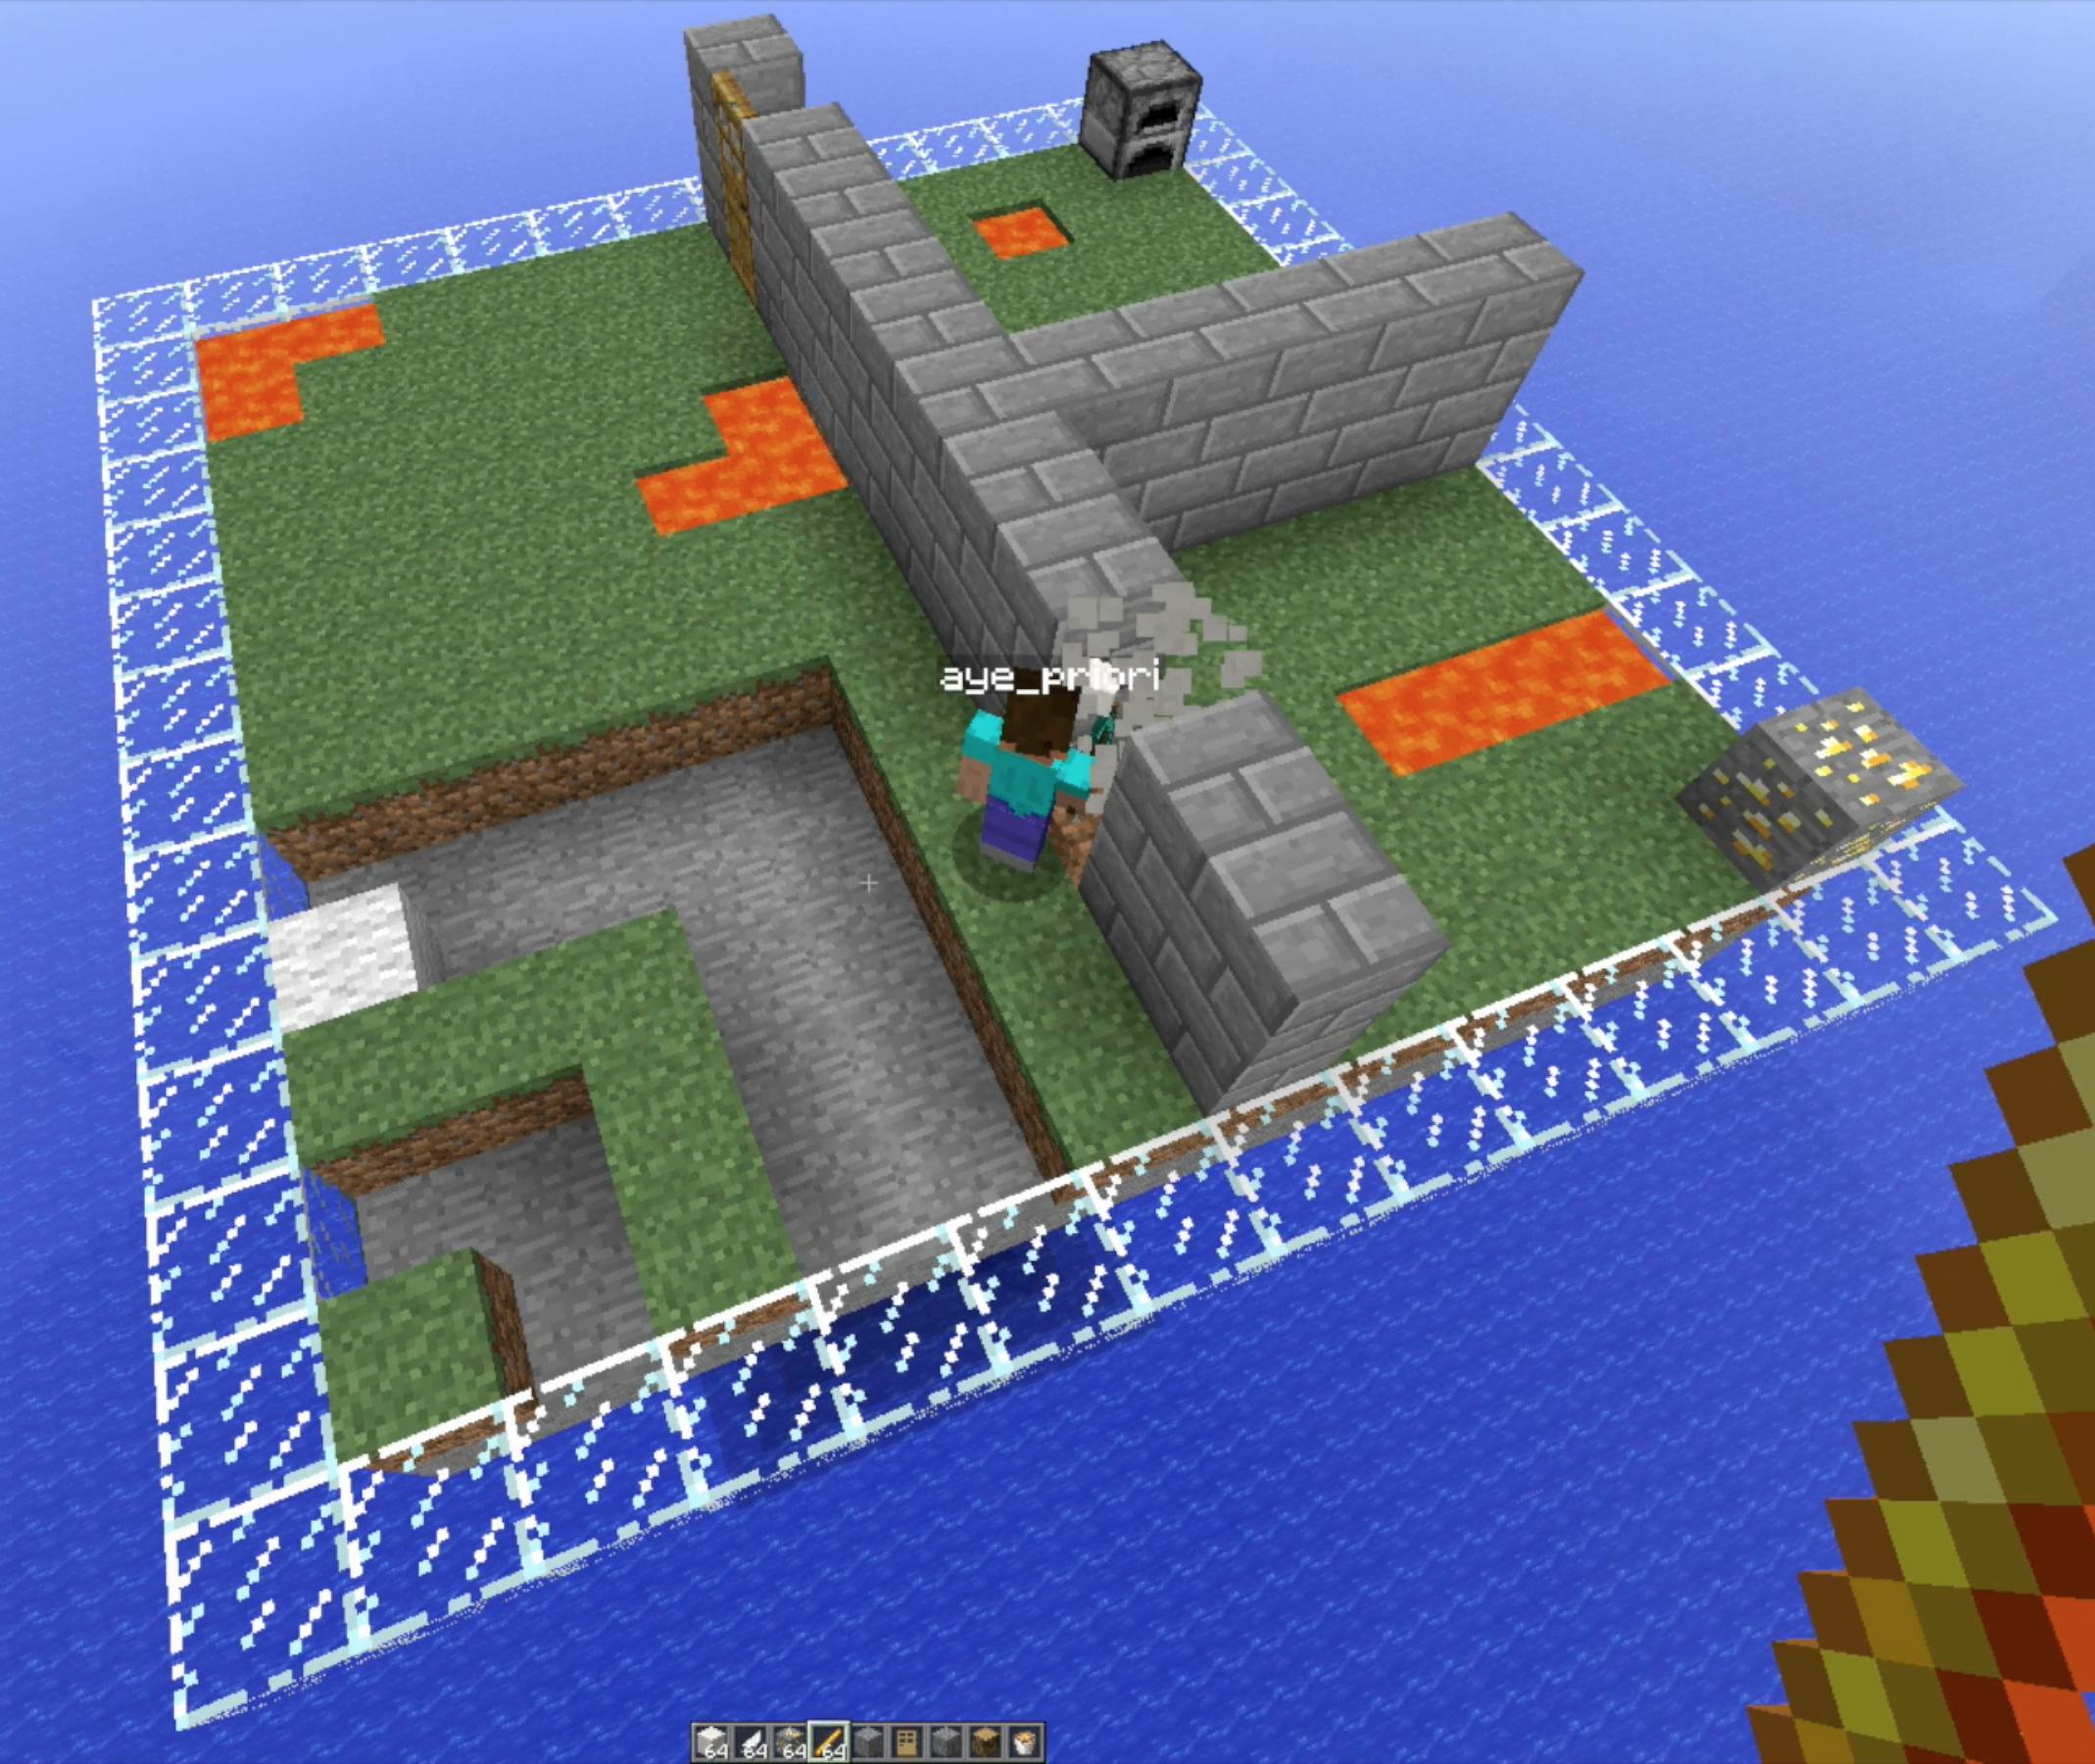
\includegraphics[width=0.24\linewidth]{figures/epicworld_2.jpg}}%
\subfigure[Collect Ore]{
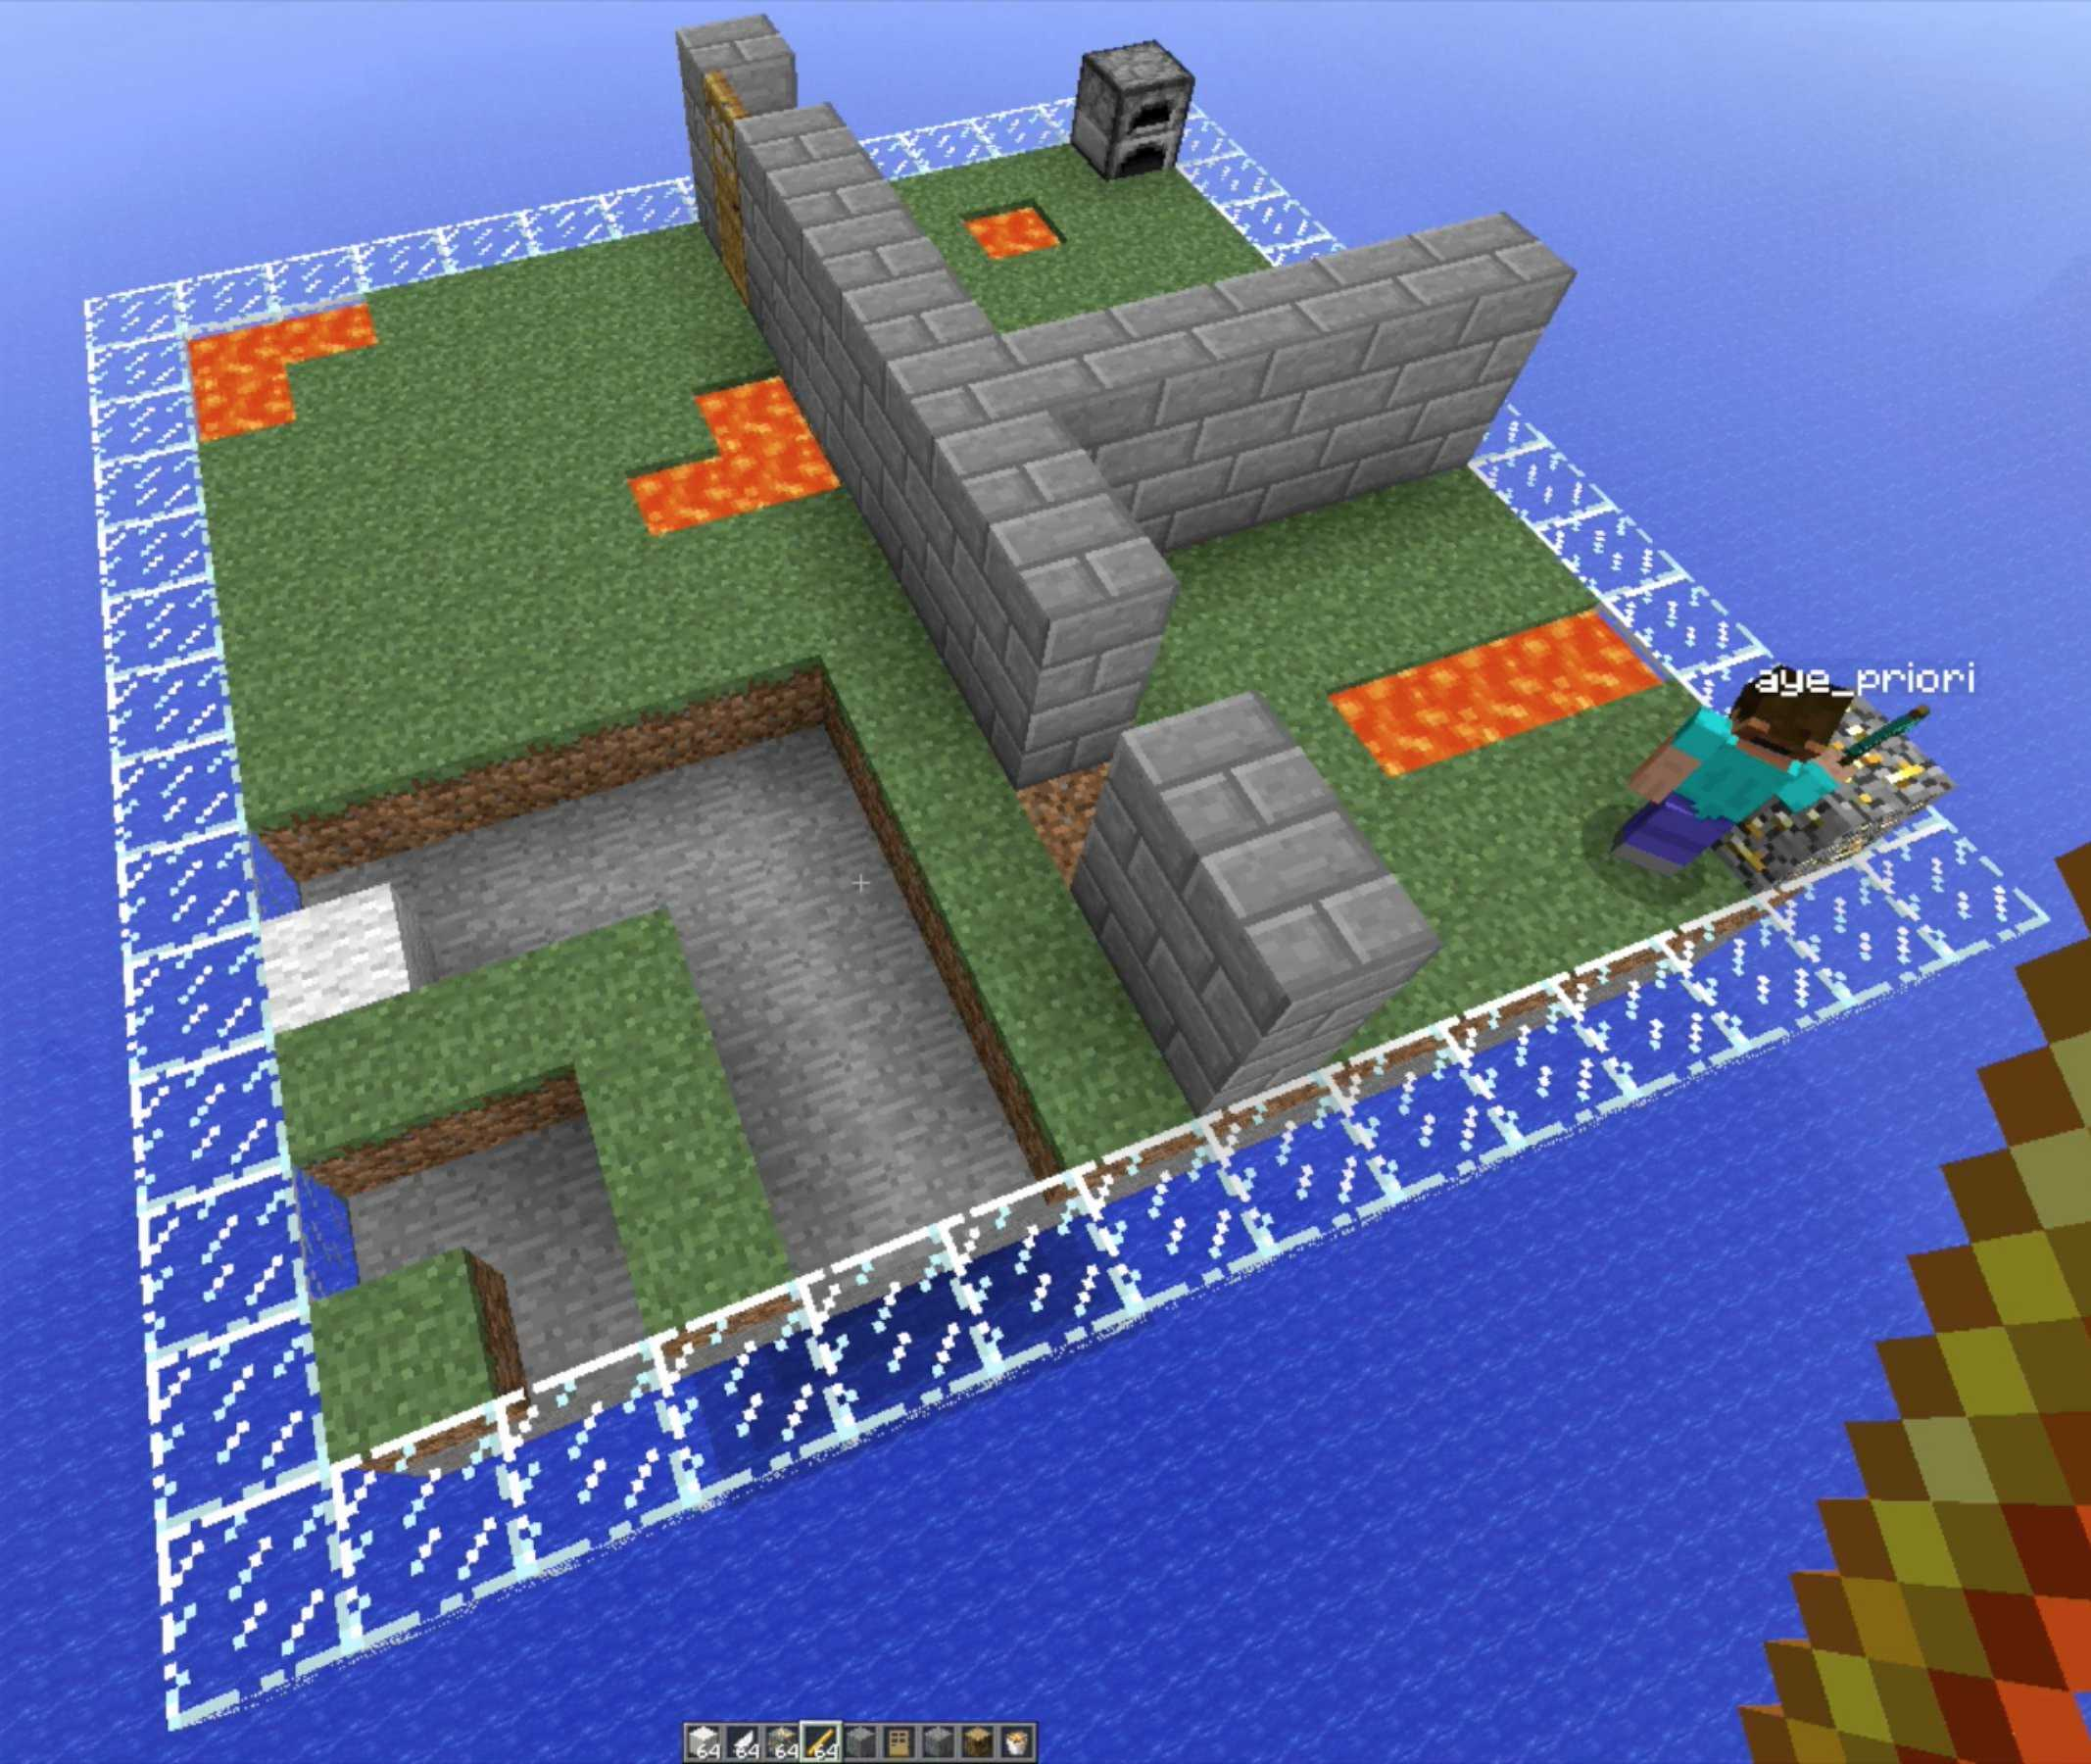
\includegraphics[width=0.24\linewidth]{figures/epicworld_3.jpg}}%
\subfigure[Smelt Ore]{
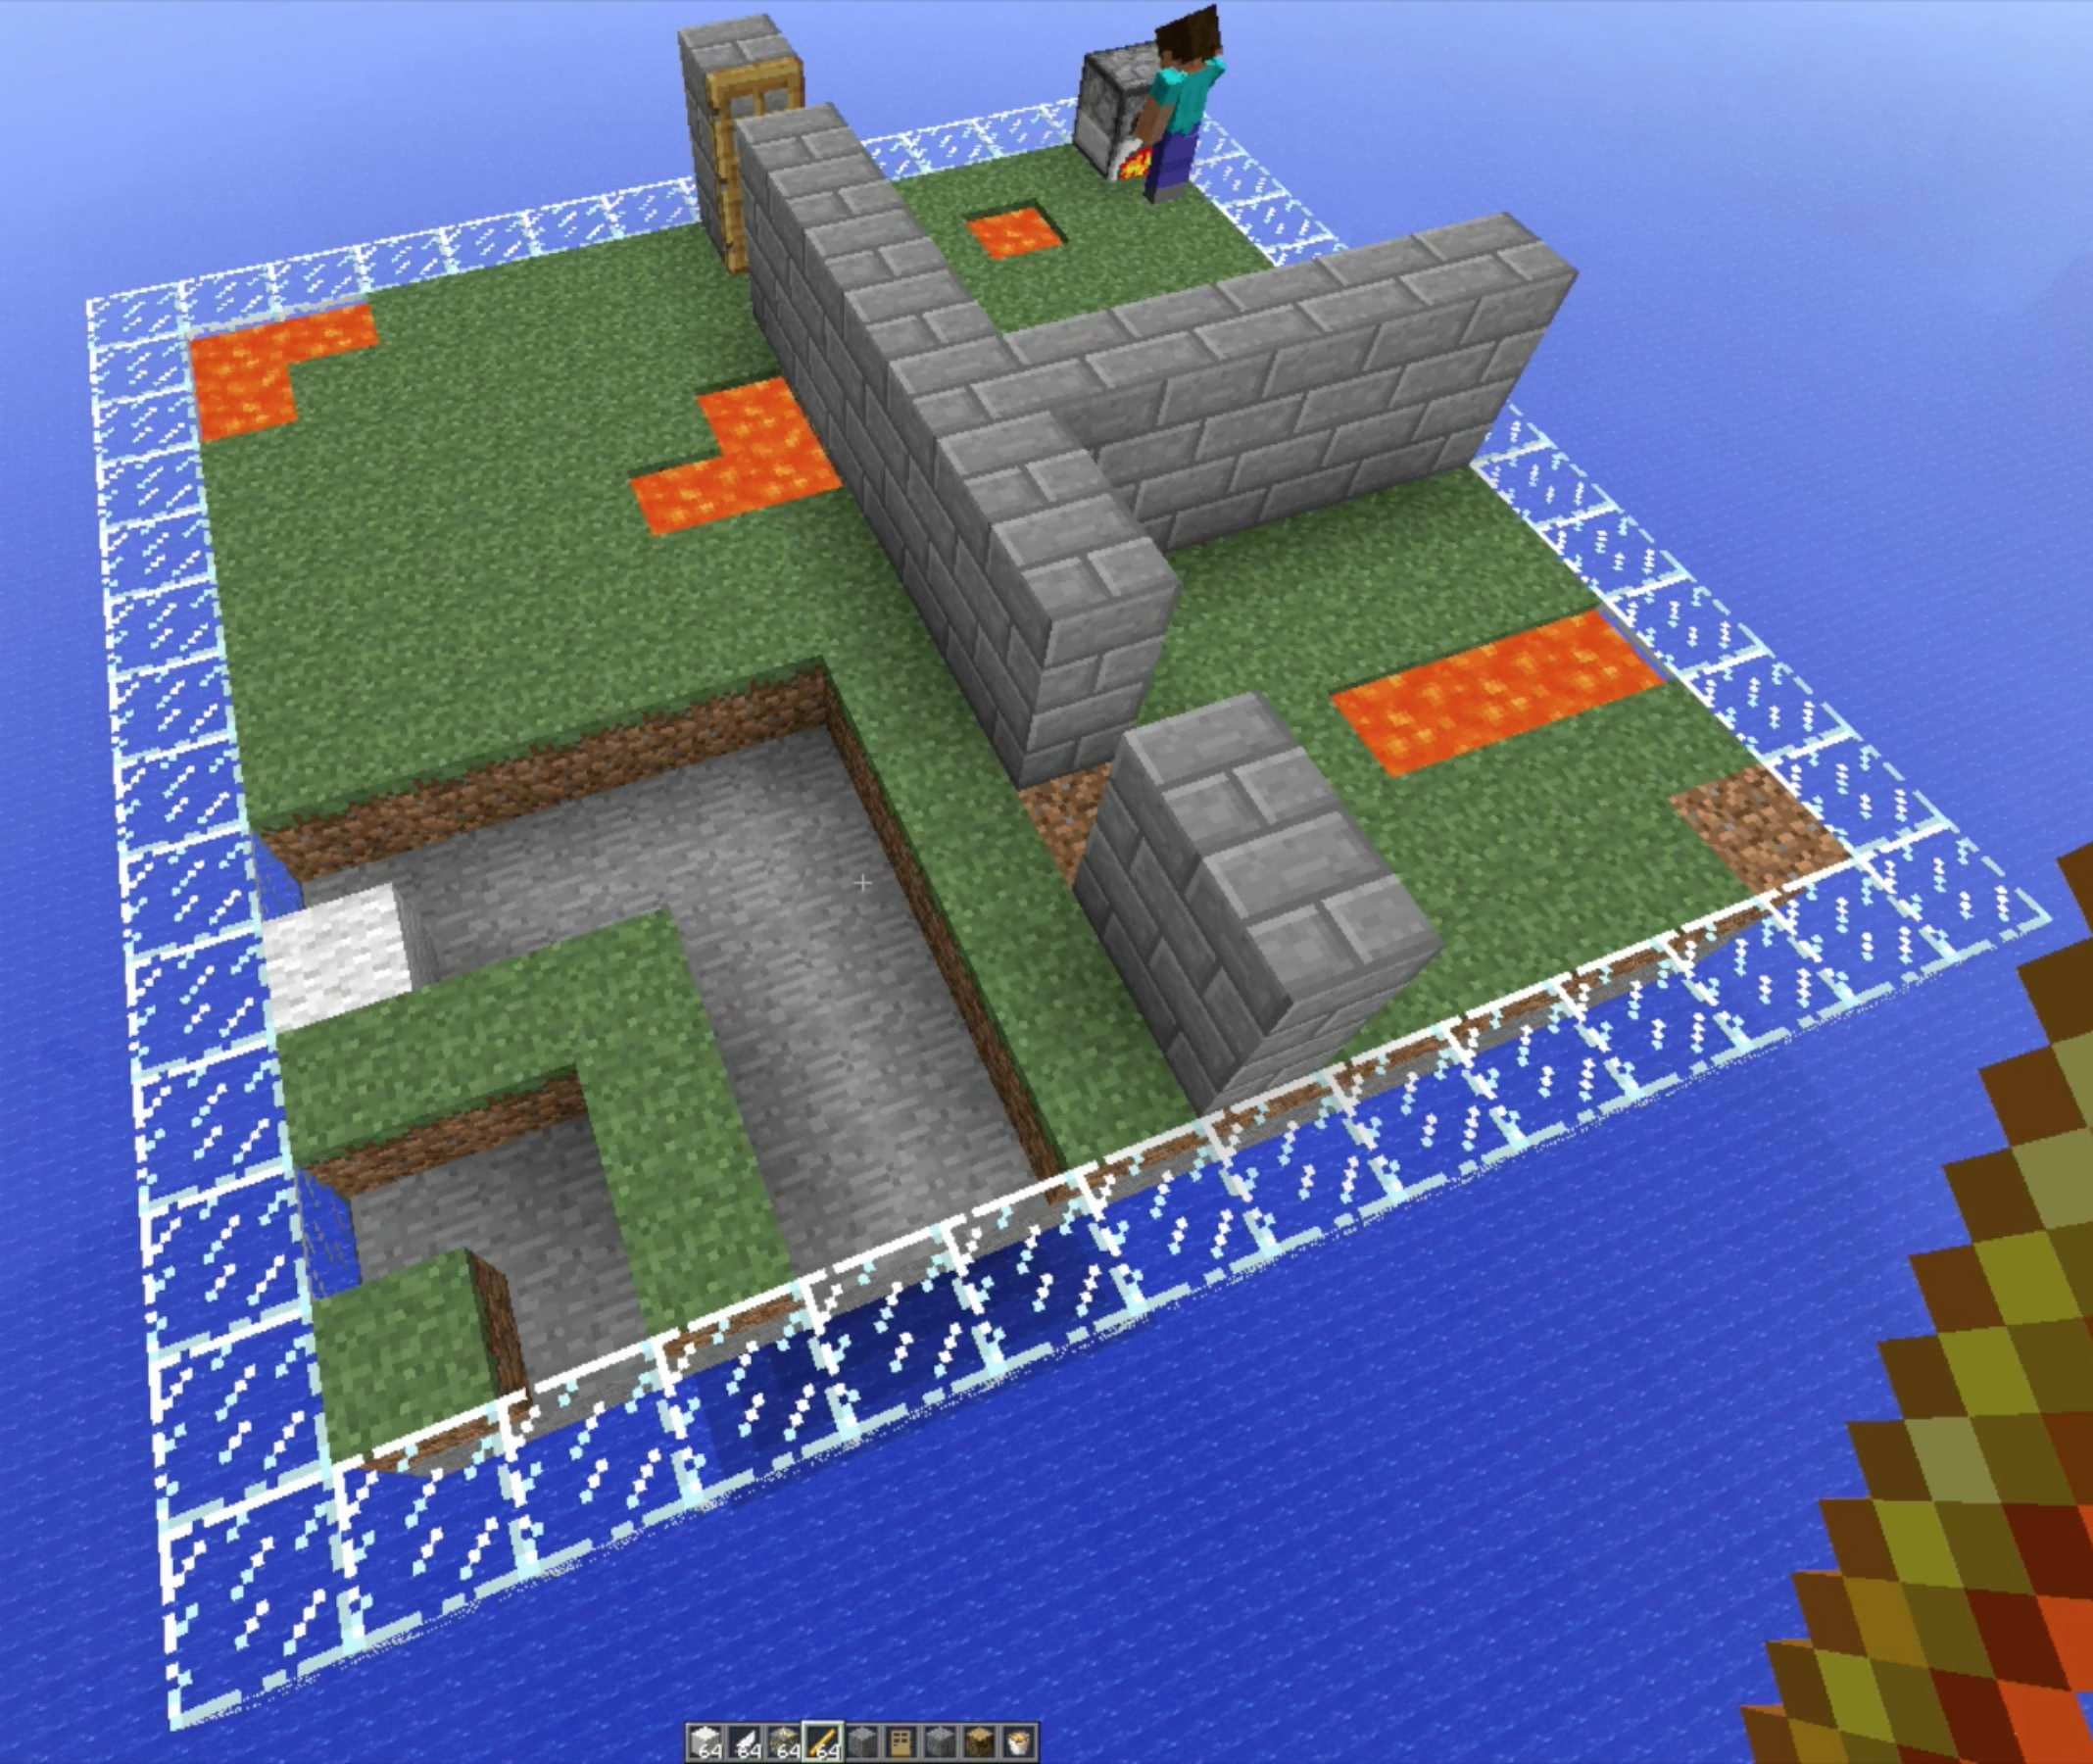
\includegraphics[width=0.24\linewidth]{figures/epicworld_4.jpg}}%
  \caption{Affordance-aware RTDP tasked with a gold-smelting task with a variety of obstacles. This planning task was
  only solved by an affordance-aware planner.}
  \label{fig:epicworld}
\end{figure*}

Minecraft serves as an effective parallel for the actual world, both
in terms of approximating the complexity and scope of planning
problems, as well as modeling the uncertainty and noise presented to a
real world agent.  For instance, robotic agents are prone to
uncertainty all throughout their system, including noise in their
sensors (cameras, LIDAR, microphones, etc.), odometry, control, and
actuation.  In order to accurately capture some of the inherent
difficulties of planning under uncertainty, the Minecraft agent's
actions were modified to have stochastic outcomes. These stochastic
outcomes may require important changes in the optimal policy in
contrast to deterministic actions, such as keeping the agent's
distance from a pit of lava. We chose to give the Minecraft agent perfect
sensor data about the Minecraft world, as that is presently beyond the focus of this
work.

\subsection{OO-MDPs}
We define affordances in terms of propositional functions on states. Our definition builds on the Object-Oriented Markov Decision Process
(OO-MDP)~\citep{diuk08}.  OO-MDPs are an extension of
the classic Markov Decision Process (MDP).  A classic MDP is a
five-tuple: $\langle \mathcal{S}, \mathcal{A}, \mathcal{T},
\mathcal{R}, \gamma \rangle$, where $\mathcal{S}$ is a state-space;
$\mathcal{A}$ is the agent's set of actions; $\mathcal{T}$ denotes
$\mathcal{T}(s' \mid s,a)$, the transition probability of an agent
applying action $a \in \mathcal{A}$ in state $s \in \mathcal{S}$ and
arriving in $s' \in \mathcal{S}$; $\mathcal{R}(s,a,s')$ denotes the
reward received by the agent for applying action $a$ in state $s$ and
and transitioning to state $s'$; and $\gamma \in [0, 1)$ is a discount
  factor that defines how much the agent prefers immediate rewards
  over distant rewards (the agent more greatly prefers to maximize
  more immediate rewards as $\gamma$ decreases).

A classic way to provide a factored representation of an MDP state is to represent
each MDP state as a single feature vector. By contrast, an OO-MDP represents the state space as a collection of objects,
$O = \{o_1, \ldots, o_o \}$.  Each object $o_i$ belongs to a
class $c_j \in  \{c_1, \ldots, c_c\}$. Every class has a set of attributes
$Att(c) = \{c.a_1, \ldots, c.a_a \}$, each of which has a domain $Dom(c.a)$ of possible values.
Upon instantiation of an object class, its attributes are given a state $o.state$
(an assignment of values to its attributes).  The underlying MDP state is the set
of all the object states: $s \in {\cal S} = \cup_{i = 1}^o \{o_i.state\}$.

There are two advantages to using an object-oriented factored state
representation instead of a single feature vector. First, different
states in the same state space may contain different numbers of
objects of varying classes, which is useful in domains like Minecraft
in which the agent can dynamically add and remove blocks to the
world. Second, MDP states can be defined invariantly to the specific
object references.  For instance, consider a Minecraft world with two
block objects, $b_1$ and $b_2$.  If the agent picked up and swapped
the position of $b_1$ and $b_2$, the MDP state before the swap and
after the swap would be the same, because the MDP state definition is
invariant to which object holds which object state. 
%This
%object reference invariance results in a smaller state space compared
%to representations like feature vectors in which changes to value
%assignments always result in a different state.

While the OO-MDP state definition is a good fit for the Minecraft
domain, our motivation for using an OO-MDP lies in the ability to
formulate predicates over classes of objects. That is, the OO-MDP
definition also includes a set of predicates ${\cal P}$ that operate
on the state of objects to provide additional high-level information
about the MDP state. 
%For example, in Figure \ref{fig:epic world}, a ${\tt
%  nearTrench}({\tt STATE})$ predicate evaluates to true when the
%singular instance of class $\texttt{AGENT}$ is directly adjacent to an
%empty location at floor level (i.e. the cell beneath the agent in some
%direction does not contain a block). 
In the original OO-MDP work,
these predicates were used to model and learn an MDP's transition
dynamics.

While an OO-MDP reduces the size of the Minecraft state space
by a significant factor, the resulting state space is still far too large to
solve with any existing (OO)-MDP solver. This is the primary motivator
for incorporating affordances as a means of reducing the amount of the
state space that an OO-MDP agent will have to explore.

% ====== Section: Affordances ======
\section{Affordances}
\label{sec:affordances}

We define an affordance $\Delta$ 
as the mapping $\langle p,g\rangle \longmapsto \mathcal{A}'$,
where:
\begin{itemize}
\item[] $\mathcal{A}' \subseteq \mathcal{A}$, a subset of the action space, representing the relevant {\it action-possibilities} of the environment.
\item[] $p$ is a predicate on states, $s \longrightarrow \{$0$, 1\}$
  representing the {\em precondition} for the affordance.
\item[] $g$ is an ungrounded predicate on states, $g$, representing a {\it lifted goal description}.
\end{itemize}
The precondition and goal description predicates refer to predicates that are defined in the OO-MDP definition. 
Using OO-MDP predicates for affordance preconditions and goal descriptions 
allows for state space independence. Thus, a planner equipped with
affordances can be used in any number of different tasks. 

\subsection{Affordance Aware Planning}
We call any planner that
uses affordances an {\it affordance-aware} planner. For a given state, 
our goal is to solve for the probability of getting a particular action set $\mathcal{A}^*$, and approximate sampling
from this distribution. This ensures that in the limit, it is possible to apply each action in each state.
\begin{equation}
\text{Pr}(\mathcal{A}^* \mid s, \Delta_0 \dots \Delta_N)
\end{equation}
We let each affordance contribute a set $\mathcal{A}'$ in each state:
\begin{align}
\text{Pr}(\mathcal{A}'_0 \cup \mathcal{A}'_N \mid s, \Delta_0 \dots \Delta_N)
\end{align}
We approximate this term assuming the sets $\mathcal{A}_i'$ are disjoint:
\begin{align}
\sum_i^K \text{Pr}(\mathcal{A}'_i \mid s, \Delta_i)
\end{align}

Given a set of $K$ domain affordances $Z = \{\Delta_1, ..., \Delta_K\}$ and a current 
agent goal condition defined with an OO-MDP predicate $G$, the action set that a 
planning algorithm considers is pruned on a state by state basis as shown in 
Algorithm~\ref{alg:prune_actions}. For instance, the affordances defined for Minecraft 
navigation problems can be used in any task regardless of the spatial size of the world, 
number of blocks in the world, and specific goal location that needs to be reached. Each 
activated affordance contributes a suggested action set, determined by Algorithm \ref{alg:get_actions}. 
We call an affordance {\it activated} when its predicate is true and the lifted goal description $g$ matches the agent's current goal.

\begin{algorithm}
  \caption{getActionsForState($state$, $Z$, $G$)}
  \begin{algorithmic}[1]
    \State $\mathcal{A}^* \leftarrow \{\}$
    \For {$\Delta \in Z$}
    \If {$\Delta.p(state)$ and $\Delta.g = G$}
    \State $\mathcal{A}^* \leftarrow \mathcal{A}^* \cup \Delta.getActions(s)$
    \EndIf
    \EndFor \\
    \Return $\mathcal{A}^*$
  \end{algorithmic}
  \label{alg:prune_actions}
\end{algorithm}

Specifically, we prune actions on a state by state basis
by initializing an empty set of actions $\mathcal{A}^*$ (line 1). The algorithm then iterates
through each of the domain affordances (lines 2-6). If the affordance
precondition ($\Delta.p$) is satisfied by some set of objects in the current state
and the affordance goal condition ($\Delta.g$) is defined with the same predicate
as the current goal (line 3), then the actions associated with the affordance ($\Delta.\mathcal{A}' = \Delta.getActions(s)$) are added to the action set $\mathcal{A}^*$ (line 4). Finally, $\mathcal{A}^*$ is returned (line 7).

\begin{figure}
\centering
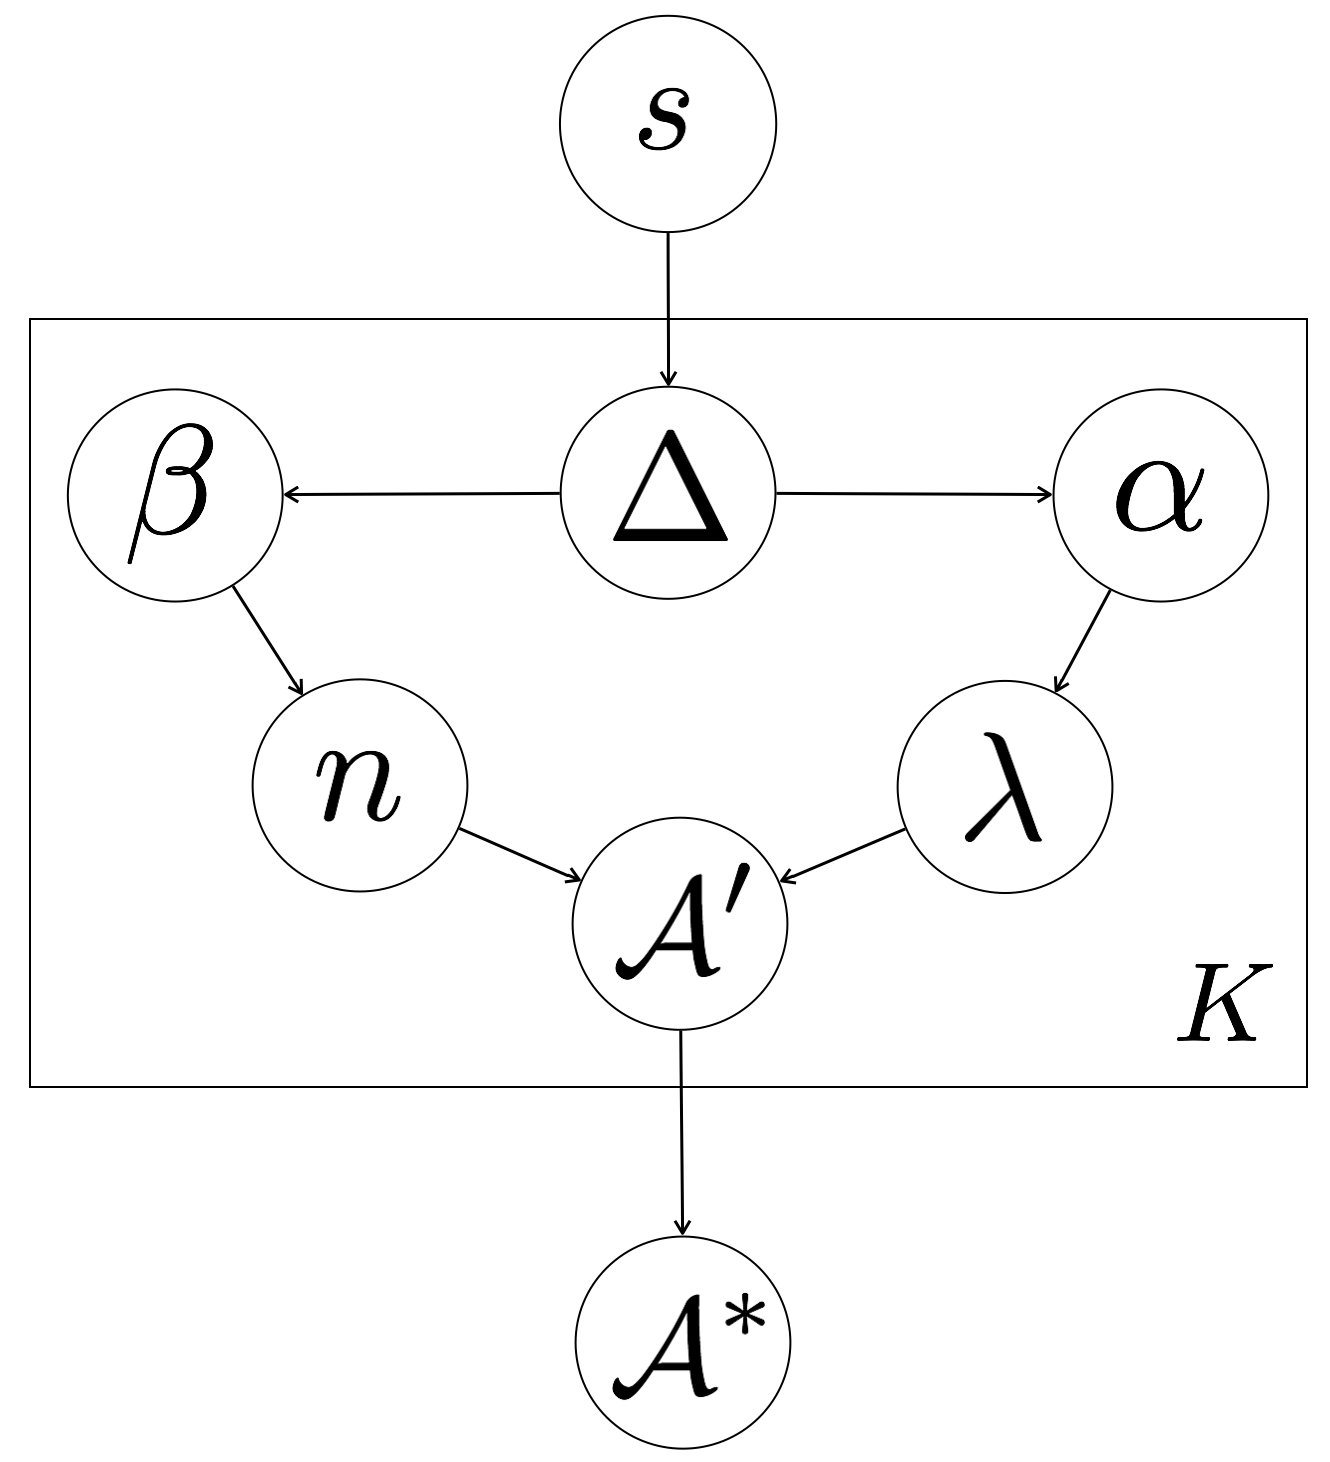
\includegraphics[scale=0.15]{figures/learn_graphical_model.png}%
  \caption{The full graphical model approximating a distribution over $\mathcal{A}^*$, the pruned action set for a given state $s$}
  \label{fig:graphical_model}
\end{figure}

Thus, for each affordance, we get an action set $\mathcal{A}'$. This 
process is outlined by Algorithm \ref{alg:get_actions}. We form a Dirichlet Multinomial
over actions ($\lambda$), and a Dirichlet over the size ($N$) of each action set:
\begin{equation}
\text{Pr}(\mathcal{A}_i \mid s,\Delta_i) = \text{Pr}(\mathcal{A}_i' \mid N, \lambda) = \text{Pr}(\lambda \mid \alpha) \cdot \text{Pr}(N \mid \beta)
\end{equation}

For a given affordance $\Delta_i$, we sample from our distribution over action set size to get a candidate action set size (lines 1-2). We then
take that many samples from our distribution over actions to get a candidate action set $\mathcal{A}'$ (lines 3-5).
\begin{align}
\text{Pr}(\lambda \mid \alpha) = DirMult(\alpha) \\
\text{Pr}(N \mid \beta) = Dir(\beta)
\end{align}

\begin{algorithm}
  \caption{$\Delta_i.getActions(s)$}
  \begin{algorithmic}[1]
    \State $\lambda \leftarrow DirMult(\Delta_i.\alpha)$
    \State $N \leftarrow Dir(\Delta_i.\beta)$
    \For {$1$ to $N$}
    \State $\Delta_i.\mathcal{A}' \leftarrow \lambda$
    \EndFor \\
    \Return $\Delta_i.\mathcal{A}'$
  \end{algorithmic}
  \label{alg:get_actions}
\end{algorithm}

Through the use of Algorithms \ref{alg:prune_actions} \& \ref{alg:get_actions}, any OO-MDP solver made be made
{\it affordance aware}. For a planner to be made affordance-aware, we require that an expert provide a set $\mathcal{P}$ of predicates
for the domain of relevance (i.e. Minecraft). Additionally, the expert must specify a set
$\mathcal{G} \subset \mathcal{P}$, that indicates which predicates may serve as goal conditions. If the expert wishes
to provide the affordances directly, they must specify the Dirichlet parameters $\alpha$ and $\beta$. Note that
in the limit, the expert may fix $\alpha$ and $\beta$ in a way that forces a given
affordance to always suggest a specific set of actions.

The real strength of our affordance formalism is that it is simple enough to learn useful affordances directly.

\subsection{Learning Affordances}

To learn affordances, we propose a scaffolded learning process that computes $\alpha$ and $\beta$ by solving OO-MDPs in small state-spaces that present similar sorts of features to the state spaces the agent might expect to see.

Given the set of predicates $\mathcal{P}$ and possible goals $\mathcal{G} \subset \mathcal{P}$, we form a set of candidate affordances $\Delta$ with every combination of $\langle p, g \rangle$, for $p \in \mathcal{P}$ and $g \in \mathcal{G}$.

Then, we randomly generate a large number of state spaces which are small 
enough to be solved using tabular methods (typically on the order of several hundred to a few thousand), 
annotated with their lifted goal description $g \in \mathcal{G}$. We solve the 
OO-MDP in each state space to find an optimal policy $\pi_j$.

For each optimal policy, we count the number of policies that used each action 
when each affordance was activated.\footnote{Recall we call an affordance {\it activated} 
when its predicate is true and the lifted goal description $g$ matches the agent's current goal.} 
These counts represent $\alpha$. Then, we count the number of unique actions used by each policy, representing $\beta$. 

% ====== Section: Experiments ======
\section{Experiments}
\label{sec:experiments}

We conducted a series of experiments in the Minecraft domain that
compared the performance of several OO-MDP solvers without affordances,
to their affordance-aware counterparts. We selected the expert
affordances from our background knowledge of the domain. Additionally, we
tested our learning procedure and compared the performance of RTDP solving the OO-MDP
with (1) No affordances, (2) Learned affordances, and (3) Expert provided affordances. We generated between 10-5000 simple state
spaces to learn on, each a $3\times3\times3$ world with randomized features based on the features of the agent's actual state space.

We gave the agent a single knowledge base of 5 types of affordances,
which are listed in Figure \ref{fig:afford_kb_exp}.  Our experiments
consisted of a variety of common tasks in Minecraft, ranging from
basic path planning, to smelting gold, to opening doors and tunneling
through walls.  We also tested each planner on worlds of varying size
and difficulty to demonstrate the scalability and flexibility of the
affordance formalism. The evaluation metric for each trial was the
number of state backups that were executed by each planning
algorithm. Value Iteration was terminated when the maximum change in
the value function was less than 0.01. RTDP terminated when the
maximum change in the value function was less than 0.01 for five
consecutive policy rollouts. In subgoal planning, the high-level
subgoal plan was solved using breadth-first search; which only took a
small fraction of the time compared to the total low-level planning
and therefore is not reported.  We used RTDP as the low-level planner
for subgoal planning.

We set the reward function to $-1$ for all transitions, except
transitions to states in which the agent was on lava, which returned 
$-200$. The goal was set to be terminal. The discount
factor was set to $\lambda = 0.99$. For all experiments, the agent was given stochastic actions. Specifically, actions associated with a direction (e.g. movement, block placement, jumping, etc.), had a small probability ($0.3$) of moving in another random direction.

\begin{figure}[b]
\begin{empheq}{align*}
\Delta_1 &= \langle nearTrench, reachGoal \rangle \longmapsto \{place, jump\} \\
\Delta_2 &= \langle onPlane, reachGoal \rangle \longmapsto \{move\} \\
\Delta_3 &= \langle nearWall,reachGoal \rangle \longmapsto \{destroy \} \\
\Delta_4 &= \langle nearFurnace, makeGold \rangle \longmapsto \{place\} \\
\Delta_5 &= \langle nearOre, makeGold \rangle \longmapsto \{destroy\}
\vspace{6 pt}
\end{empheq}
\caption{The five affordance types used in expert experiments.}
\label{fig:afford_kb_exp}
\end{figure}

% ==== SECTION: RESULTS ====
\section{Results}
\label{sec:results}

Table~\ref{table:hard-results} shows the number of Bellman updates required when solving the OO-MDP with conventional methods (left column)
compared to solving the OO-MDP with an Affordance-Aware method (right column).  The
affordance aware methods significantly outperformed their unaugmented
counterparts in all of these experiments. These
results, while unsurprising, concretely demonstrate that a small set of affordances prune away many useless actions across many different types of Minecraft tasks. 

\begin{table}
\centering
\caption{Expert Affordance Results: Avg. Number of Bellman Updates per converged policy}
\begin{tabular}{ l || c c | c c | c  c }
  & VI & A-VI & RTDP & A-RTDP & SG & A-SG \\ \hline
  \texttt{4TRENCH} 		&	71604 		& 	{\bf 100} 		& 	836 		& 	{\bf 152} 		&	1373 	& 	{\bf 141}  			\\
  \texttt{6TRENCH} 		&	413559 	 	& 	{\bf 366}  		& 	4561 	& 	{\bf 392} 		&	28185 	& 	{\bf 547}  \\
  \texttt{8TRENCH} 		&	1439883 		& 	{\bf 904}		& 	18833	& 	{\bf 788}		&	15583	& 	{\bf 1001} 			\\
  \texttt{DOOR} 		&	861084 	 	& 	{\bf 4368}		& 	12207	& 	{\bf 1945}		&	6368		& 	{\bf 1381}	\\
  \texttt{LAVA}  		&	413559 		& 	{\bf 366}	 	& 	4425 	& 	{\bf 993}  		&	25792	& 	{\bf 597}   \\
  \texttt{TUNNEL}  		&	203796 		& 	{\bf 105}		& 	26624	& 	{\bf 145}  		&	5404 	& 	{\bf 182}	\\
  \texttt{GOLD}  		&	16406		& 	{\bf 962}		& 	7738 	& 	{\bf 809}  		&	7412 	& 	{\bf 578}
\end{tabular}
\label{table:hard-results}
\end{table}

Table \ref{table:learned-results} indicates the average number of Bellman updates required by RTDP to solve the OO-MDP
in each of the four candidate worlds. The learned affordances clearly improved on standard RTDP by a significant margin, though
there is still a substantial gap between the learned affordance performance and that of the expert affordances. This indicates that
there is still room for improvement in the learning process.
\begin{table}
\centering
\caption{Learned Affordance Results: Avg. Number of Bellman Updates per converged policy}
\begin{tabular}{ l || c c c }
  & No Affordances & Learned & Expert  \\ \hline
  \texttt{Tiny World}  		& 	879		&	414	&	 94	\\
  \texttt{Small World}  	& 	1460		&	802	&	321  \\
  \texttt{Medium World}  	& 	3993		&	2412	&	693  \\
  \texttt{Large World}  	& 	8344		&	5100	&	1458
\end{tabular}
\label{table:learned-results}
\end{table}

Figure \ref{fig:training_results} demonstrates the added effect of more training data. The chart indicates that the more time invested into learning affordances for a knowledge base, the faster an OO-MDP may be solved. In these experiments, we tested on map types that mimicked the features of the worlds generated during training, but this process could be extended to allow for scaffolded learning and more complicated maps (such as the gold smelting task in Figure \ref{fig:epicworld}). The averages reported are from solving the OO-MDP 20 times for each world, with each knowledge base. There was a negligible difference in the quality of the policies generated.
\begin{figure}[b]
\centering
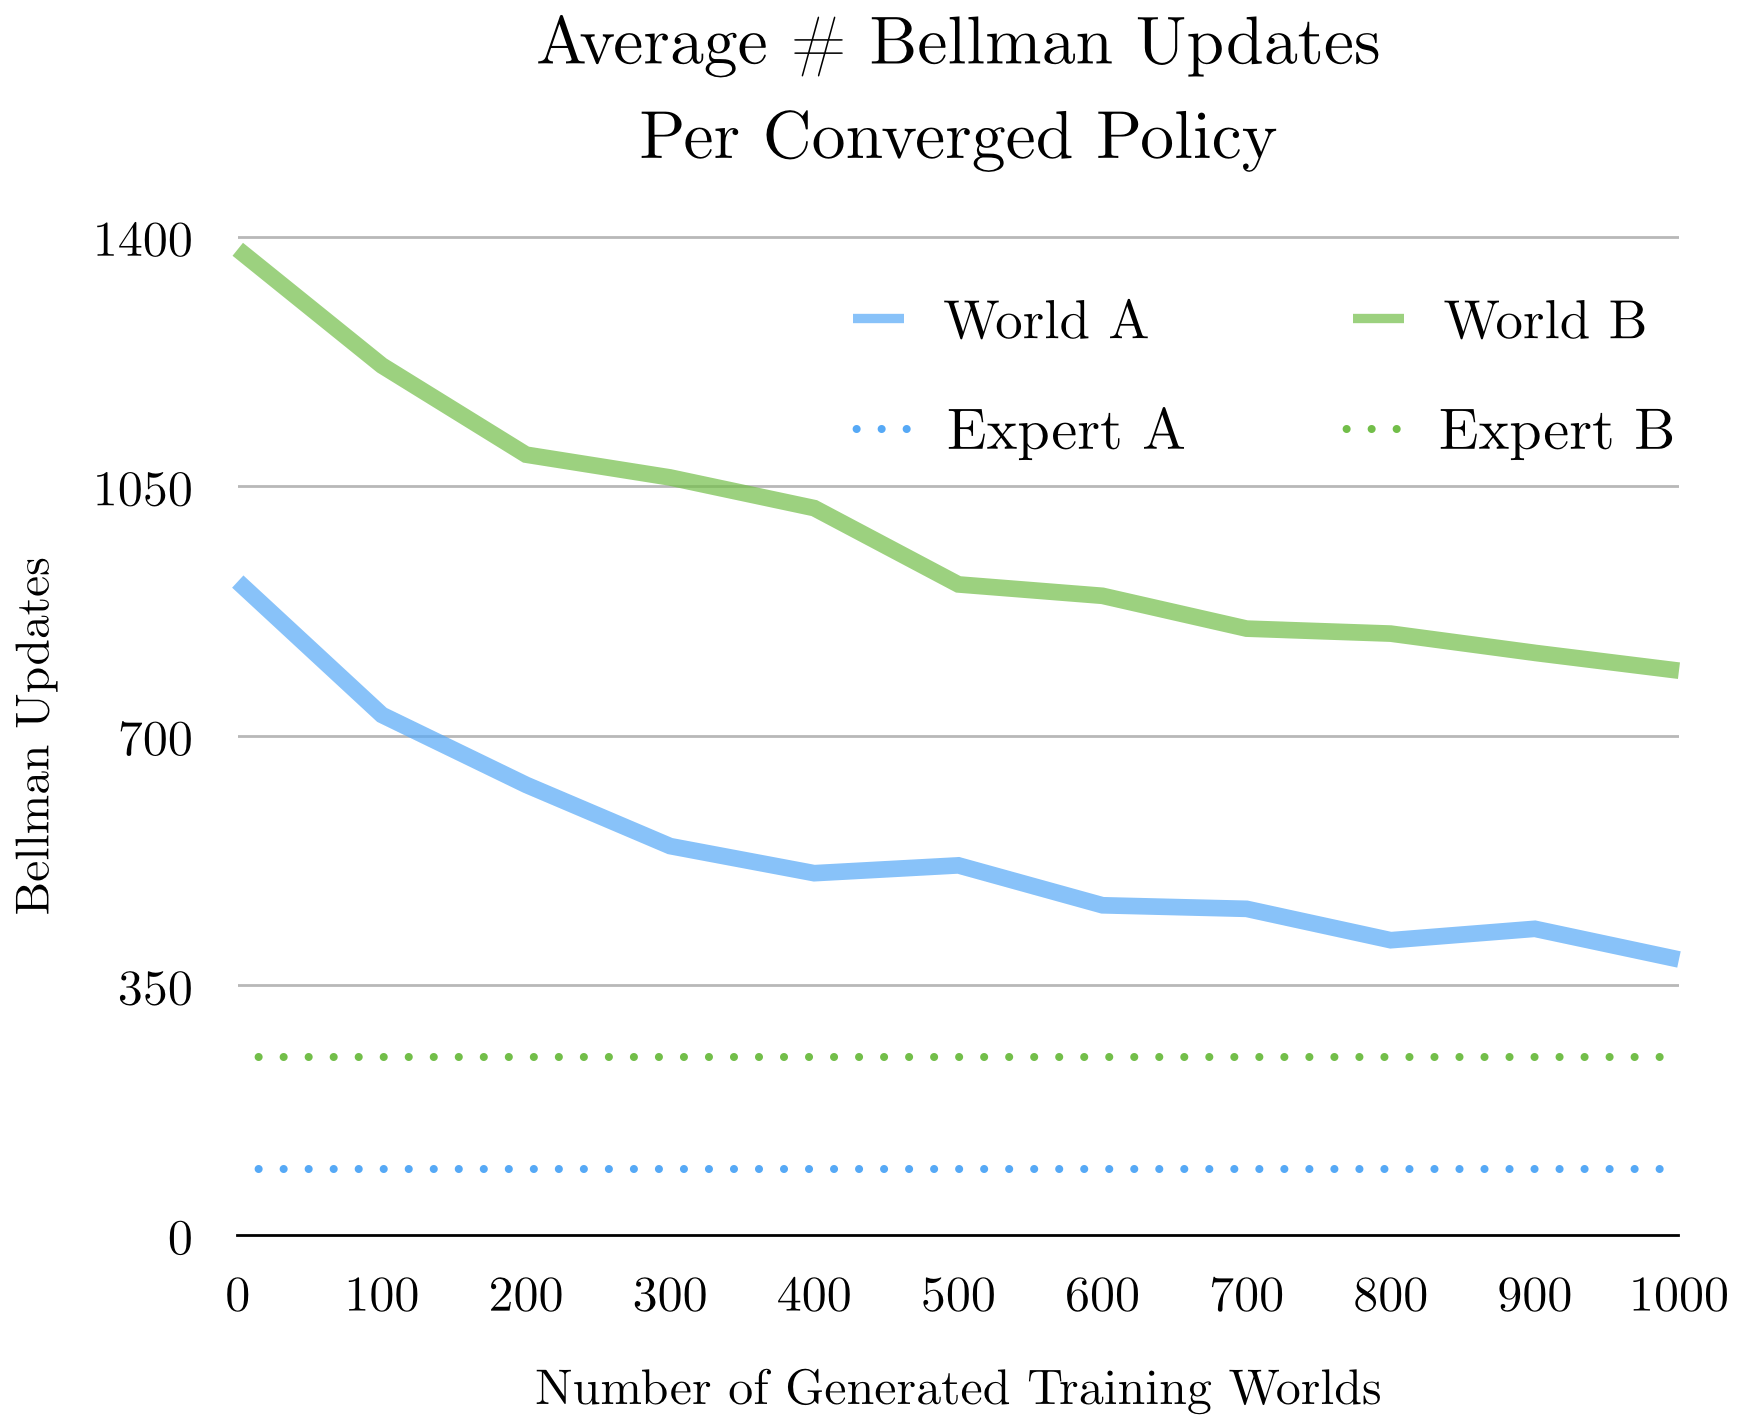
\includegraphics[scale=0.25]{figures/training_results.png}%
  \caption{The effectiveness of added training data on solving an OO-MDP.}
  \label{fig:training_results}
\end{figure}

% ====== Section: Related Work ======
\section{Related Work}
\label{sec:related-work}

In this section, we discuss the differences between
affordance-aware planning and other forms of knowledge that
have been used to accelerate planning.

% --- Subsection: Temporarily Extended Actions ---
\subsection{Temporarily Extended Actions}
Temporally extended actions are actions that the agent can
select like any other action of the domain, except executing them
results in multiple primitive actions being executed in
succession. Two common forms of temporally extended actions are {\em
  macro-actions}~\citep{hauskrecht98} ~and {\em options}~\citep{sutton99}. 
Macro-actions are actions that always
execute the same sequence of primitive actions. Options are defined
with high-level policies that accomplish specific sub tasks. For
instance, when an agent is near a door, the agent can engage the
`door-opening-option-policy', which switches from the standard
high-level planner to running a policy that is hand crafted to open
doors. 

Although the classic options framework is not generalizable to different state spaces,
creating {\em portable} options is a topic of active research~\citep{konidaris07,konidaris2009efficient,Ravindran03analgebraic,croonenborghs2008learning,andre2002state,konidaris2012transfer}.

Given the potential for unhelpful temporally extended actions to negatively impact planning time~\citep{Jong:2008zr}, we believe combing affordances with temporally extended actions
may be especially valuable because it will restrict the set of temporally extended actions to those
useful for a task. In the future, we plan to explore the benefit from combining
these approaches.

% --- Subsection: Action Pruning ---
\subsection{Action Pruning}

Sherstov and Stone~\citep{sherstov2005improving} considered MDPs with a very large action set and for which the action
set of the optimal policy of a source task could be transferred to a new, but similar, target
task to reduce the learning time required to find the optimal policy in the target task.

The main difference between our affordance-based action set pruning and this action transfer
work is that affordances prune away actions on a state by state basis, where
as the learned action pruning is on per task level. Further, with lifted goal descriptions, affordances may be attached to subgoal planning for a significant
benefit in planning tasks where complete subgoal knowledge is known (or may be inferred).

Rosman and Ramamoorthy~\citep{rosman2012good} provide a method for learning action priors over a set of related tasks. Specifically, they compute a Dirichlet distribution over actions by extracting the frequency that each action was optimal in each state for each previously solved task.

There are a few limitations of the actions priors work that affordance-aware planning does not possess: (1) the action priors can only be used with planning/learning algorithms that work well with an $\epsilon$-greedy rollout policy; (2) the priors are only utilized for fraction $\epsilon$ of the time steps, which is typically quite small; and (3) as variance in tasks explored increases, the priors will become more uniform. In contrast, affordance-aware planning can be used in a wide range of planning algorithms, benefits from the pruned action set in every time step, and the affordance defined lifted goal-description enables higher-level reasoning such as subgoal planning.

% --- Subsection: Temporal Logic ---
\subsection{Temporal Logic}

Bacchus and Ady~\citep{Bacchus95usingtemporal, Bacchus99usingtemporal} provided
planners with domain dependent knowledge in the form of a first-order version of linear
temporal logic (LTL), which they used for control of a forward-chaining planner - often
achieving polynomial time planning in exponential space. With this methodology, 
\textsc{Strips} style planner may be guided through the search space by checking 
whether candidate plans do not falsify a given knowledge base of LTL formulas.

While this approach is theoretically sound and has achieved empirical success, its main drawback is the complexity of its knowledge. The primary difference between this body of work and our own is that the affordance formalism may be learned, while LTL formulas are far too complicated to learn effectively.

% --- Subsection: Heuristics ---
\subsection{Heuristics}
Heuristics in MDPs are used to convey information about the value of a given state or state-action pair with respect to the task being solved and typically take the form of either {\em value function initialization},
or {\em reward shaping}. Initializing the value function to an admissible close approximation of the optimal value function has been shown to be effective for LAO* and RTDP~\citep{Hansen:1999qf}.

Reward shaping is an alternative approach to providing heuristics. The planning algorithm uses a modified version of the reward function that returns larger rewards for state-action pairs that are expected to be useful, but does not guarantee convergence to an optimal policy unless certain properties of the shaped reward are satisfied~\citep{potshap}.

A critical difference between heuristics and affordances is that heuristics are highly dependent on the reward function and state space of the task being solved, whereas affordances are state independent and transferable between different reward functions. However, if a heuristic can be provided, the combination of heuristics and affordances may even more greatly accelerate planning algorithms than either approach alone.

% ====== Section: Conclusion ======
\section{Conclusion}
\label{sec:conclusion}

We proposed a novel approach to representing knowledge in terms of
{\em affordances}~\citep{gibson77} that allows an agent to efficiently
prune its action space based on domain knowledge. This led to the 
proposal of affordance-aware planners, which improve on classic planners
by providing a significant reduction in the number of state-action pairs the
agent needs to evaluate in order to act optimally. We demonstrated the efficacy 
as well as the portability of the affordance model by comparing standard paradigm
planners to their affordance-aware equivalents in a series of challenging planning tasks in the Minecraft
domain.

Further, we designed a full learning process that allows an agent to autonomously learn useful affordances.
We provided preliminary results indicating the effectiveness of the learned affordances, suggesting that
the agent may be able to learn to tackle new types of problems on its own.

In the future, we hope to increase our coverage of Minecraft to solve even more difficult planning problems, as well as
extending this approach beyond the Minecraft domain and onto actual robots, and other games (i.e. Atari). We also hope
to learn subgoals from text for use in forming a high level plan in conjunction with our affordance formalism.

%\section{RSS citations}

%Please make sure to include \verb!natbib.sty! and to use the
%\verb!plainnat.bst! bibliography style. \verb!natbib! provides additional
%citation commands, most usefully \verb!\citet!. 
%  
%\subsection{RSS Hyperlinks}
%
%This year, we would like to use the ability of PDF viewers to interpret
%hyperlinks, specifically to allow each reference in the bibliography to be a
%link to an online version of the reference. 
%As an example, if you were to cite ``Passive Dynamic Walking''
%\cite{McGeer01041990}, the entry in the bibtex would read:
%
%{\small
%\begin{verbatim}
%@article{McGeer01041990,
%  author = {McGeer, Tad}, 
%  title = {\href{http://ijr.sagepub.com/content/9/2/62.abstract}{Passive Dynamic Walking}}, 
%  volume = {9}, 
%  number = {2}, 
%  pages = {62-82}, 
%  year = {1990}, 
%  doi = {10.1177/027836499000900206}, 
%  URL = {http://ijr.sagepub.com/content/9/2/62.abstract}, 
%  eprint = {http://ijr.sagepub.com/content/9/2/62.full.pdf+html}, 
%  journal = {The International Journal of Robotics Research}
%}
%\end{verbatim}
%}
%\noindent
%and the entry in the compiled PDF would look like:
%
%\def\tmplabel#1{[#1]}
%
%\begin{enumerate}
%\item[\tmplabel{1}] Tad McGeer. \href{http://ijr.sagepub.com/content/9/2/62.abstract}{Passive Dynamic
%Walking}. {\em The International Journal of Robotics Research}, 9(2):62--82,
%1990.
%\end{enumerate}
%%
%where the title of the article is a link that takes you to the article on IJRR's website. 
%
%
%Linking cited articles will not always be possible, especially for
%older articles. There are also often several versions of papers
%online: authors are free to decide what to use as the link destination
%yet we strongly encourage to link to archival or publisher sites
%(such as IEEE Xplore or Sage Journals).  We encourage all authors to use this feature to
%the extent possible.



%\section*{Acknowledgments}

%% Use plainnat to work nicely with natbib. 
{\small
\bibliographystyle{plainnat}
\bibliography{main}
}
\end{document}


